\chapter{Ekosistem dan Struktur Trofik}\label{ch:b1:ecosystem-organization}

Sebuah mata air di sebuah dataran batu kapur mencurahkan air yang
begitu jernih sehingga tiap tumbuhan, ikan dan kura-kura di dalamnya
dapat dihitung dari sebuah perahu. Cahaya matahari jatuh pada rumput
belutnya sebesar \qty{1.7}{} juta kilokalori tiap meter persegi
setahun; rumputnya menyimpan satu persennya; siput dan kura-kura yang
memakan rumputnya memperoleh seperenamnya; ikan yang memakan siputnya
sepersepuluhnya lagi; dan satu bangau di puncaknya hidup dari
seperseratus ribu apa yang jatuh pada airnya. Tiap \omterm{def:b1:ecosystem-organization:ecosystem}{ekosistem} dibangun
demikian: sebuah arus energi yang masuk sekali, berpindah dari pemakan
ke yang dimakan, lalu pergi sebagai panas, sementara materi yang
digerakkannya didaur ulang. Bab ini mendefinisikan \omterm{def:b1:ecosystem-organization:ecosystem}{ekosistem} dan
bagiannya, \omterm{def:b1:ecosystem-organization:niche}{relung} yang ditempati tiap spesiesnya, \omterm{def:b1:ecosystem-organization:trophic}{aras trofik} dan
\omterm{def:b1:ecosystem-organization:foodweb}{jaring makanan} yang lewatnya energinya mengalir, produktivitas yang
menetapkan ukuran keseluruhannya, serta cara menghitung berapa banyak
macam makhluk yang hidup di dalamnya.

\section{Ekosistem dan relung}

\begin{definition}[Ekosistem, biotop, komunitas]\label{def:b1:ecosystem-organization:ecosystem}
\index{ekosistem}\index{biotop}\index{komunitas}
Yang disebut \emph{ekosistem} adalah himpunan \omterm{def:b1:organism-environment:organism}{organisme} yang hidup di
sebuah tempat tertentu bersama \omterm{def:b1:organism-environment:organism}{lingkungan} fisik yang ditempati dan
dipertukarkannya: \emph{komunitas} (atau biosenosis) --- seluruh
\omterm{def:b1:populations:population}{populasi} seluruh spesiesnya --- dan \emph{biotop} --- tanah, air,
udara, cahaya dan iklimnya. Batasnya dipilih menurut pertanyaannya:
sebatang kayu lapuk, sebuah kolam, sebuah hutan, sebuah cekungan
samudra, seluruh biosfer. Sebuah ekosistem adalah sebuah \omterm{def:b1:organism-environment:organism}{sistem
terbuka} (\cref{ch:b1:organism-environment}): energi mengalir
melewatinya, materi berdaur di dalamnya dan melintasi batasnya, dan
strukturnya adalah pola siapa memakan siapa.
\end{definition}

\begin{definition}[Habitat, relung]\label{def:b1:ecosystem-organization:niche}
\index{relung ekologi}\index{habitat}
\emph{Habitat} sebuah spesies adalah tempat ia hidup; \emph{relung}nya
adalah cara ia hidup: seluruh himpunan keadaan yang ditoleransinya dan
sumber daya yang dipakainya --- suhu, kelembapan, cahaya, makanan,
waktu kegiatan, tempat bersarang --- masing-masing sebuah dimensi yang
di sepanjangnya spesiesnya menempati sebuah jangkau. Yang disebut
\emph{relung dasar} adalah jangkau yang dapat ditempatinya sendirian;
\emph{relung nyata} adalah bagian yang benar-benar ditempatinya dengan
hadirnya pesaing dan pemangsanya
(\cref{ch:b1:species-interactions}). Dua spesies dengan relung yang
sama tak dapat hidup berdampingan di satu tempat untuk waktu lama;
relung spesies yang berdampingan berbeda, dan \omterm{def:b1:ecosystem-organization:ecosystem}{komunitasnya} adalah
sehimpunan relung yang dipaskan bersama.
\end{definition}

\begin{omfigure}
\begin{tikzpicture}[font=\footnotesize, >=Stealth, line cap=round]
  \draw[->, thick] (0,0) -- (7.4,0) node[below left] {suhu};
  \draw[->, thick] (0,0) -- (0,5.2) node[below right, rotate=90, anchor=south east] {};
  \node[rotate=90, anchor=south] at (-0.4,2.6) {ukuran mangsa};
  \draw[thick, omDef, fill=omDef!18] (3.6,2.6) ellipse (2.8 and 1.9);
  \node[omDef!80!black, anchor=south] at (2.5,3.7) {relung dasar};
  \draw[thick, omThm, fill=omThm!25] (2.9,2.3) ellipse (1.6 and 1.2);
  \node[omThm!80!black] at (2.9,2.3) {relung nyata};
  \draw[thick, omProp, fill=omProp!25, opacity=0.8] (5.6,3.4) ellipse (1.5 and 1.1);
  \node[omProp!80!black, align=center] at (5.6,3.4) {relung\\ pesaingnya};
  \node[anchor=north, align=center, gray] at (3.7,-0.5) {dua di antara banyak dimensi sebuah relung; pesaingnya menyingkirkan spesiesnya dari tumpang tindihnya};
\end{tikzpicture}

{\small \omterm{def:b1:ecosystem-organization:niche}{Relung} sebagai sebuah volume dalam sebuah ruang keadaan dan
sumber daya, yang dua dimensinya digambar. \omterm{def:b1:ecosystem-organization:niche}{Relung} dasarnya adalah apa
yang dapat ditempati sebuah spesies; \omterm{def:b1:ecosystem-organization:niche}{relung} nyatanya adalah apa yang
ditinggalkan pesaingnya baginya.}
\end{omfigure}

\begin{example}[Lima burung pengicau dalam satu cemara]\label{ex:b1:ecosystem-organization:warblers}
Lima spesies burung pengicau kecil pemakan serangga bersarang dalam
hutan cemara yang sama lalu memakan serangga yang sama; ketika diamati
dengan saksama, masing-masing mencari makan di bagian pohon yang
berbeda --- puncak pohonnya, jarum baru di luarnya, cabang tengahnya,
\omterm{def:b1:flowering-plant-organization:organs}{batang} dan cabang bawahnya, tanah di bawahnya --- dan pada ketinggian
serta waktu yang berbeda. \omterm{def:b1:ecosystem-organization:niche}{Habitatnya} satu; \omterm{def:b1:ecosystem-organization:niche}{relungnya} lima, dan hutannya
memuat lima spesies padahal makanannya saja akan menyarankan satu.
\end{example}

\section{Struktur trofik}

\begin{definition}[Produsen, konsumen, pengurai]\label{def:b1:ecosystem-organization:trophic}
\index{aras trofik}\index{produsen}\index{konsumen}\index{pengurai}
\omterm{def:b1:organism-environment:organism}{Organisme} sebuah \omterm{def:b1:ecosystem-organization:ecosystem}{ekosistem} dikelompokkan menurut apa yang dimakannya
menjadi \emph{aras trofik}. \emph{Produsen} (autotrof: tumbuhan, alga,
sianobakteri, bakteri kemosintetik) membuat bahan organik dari yang
anorganik; keduanya adalah aras pertamanya. \emph{Konsumen}
memakannya: \emph{konsumen primer} (herbivora) memakan produsennya,
\emph{konsumen sekunder} (karnivora) memakan herbivoranya,
konsumen \emph{tersier} memakan karnivoranya; omnivora makan pada
beberapa arasnya. \emph{Pengurai} (bakteri, jamur) dan
\emph{detritivor} (cacing tanah, kutu kayu, kumbang tinja) hidup dari
bahan mati dan sampah dari tiap arasnya, lalu mengembalikan mineralnya
ke tanah dan airnya untuk diserap produsennya lagi --- pautan yang
menutup daur materinya.
\end{definition}

\begin{definition}[Rantai makanan, jaring makanan]\label{def:b1:ecosystem-organization:foodweb}
\index{rantai makanan}\index{jaring makanan}
Yang disebut \emph{rantai makanan} adalah sebuah urutan \omterm{def:b1:organism-environment:organism}{organisme} yang
masing-masing memakan yang sebelumnya: rumput, belalang, katak, ular,
elang. Dalam sebuah \omterm{def:b1:ecosystem-organization:ecosystem}{komunitas} nyata tiap spesies memakan beberapa dan
dimakan beberapa, dan rantainya saling mengunci menjadi sebuah
\emph{jaring makanan}, yang panahnya menunjuk dari yang dimakan ke
pemakannya --- pada arah energinya. Rantainya pendek: jarang lebih
daripada empat atau lima pautan, karena sebuah sebab yang diberikan
bagian berikutnya.
\end{definition}

\begin{omfigure}
\begin{tikzpicture}[font=\footnotesize, >=Stealth, line cap=round,
  sp/.style={draw, thick, rounded corners=3pt, inner sep=3pt, align=center, fill=white}]
  \node[sp, fill=omExo!20] (grass) at (1.5,0) {rumput belut, alga};
  \node[sp, fill=omExo!20] (det) at (6.5,0) {detritus};
  \node[sp, fill=omProp!20] (snail) at (0,2.0) {siput};
  \node[sp, fill=omProp!20] (insect) at (2.6,2.0) {larva serangga};
  \node[sp, fill=omProp!20] (turtle) at (5.0,2.0) {kura-kura};
  \node[sp, fill=omProp!20] (shrimp) at (7.6,2.0) {udang, cacing};
  \node[sp, fill=omThm!20] (sunfish) at (1.3,4.0) {ikan matahari};
  \node[sp, fill=omThm!20] (catfish) at (6.4,4.0) {ikan lele};
  \node[sp, fill=omDef!25] (bass) at (2.8,5.8) {ikan bass};
  \node[sp, fill=omDef!25] (heron) at (6.0,5.8) {bangau};
  \node[sp, fill=gray!20] (dec) at (10.2,1.0) {bakteri, jamur\\ (pengurai)};
  \draw[->, thick] (grass) -- (snail); \draw[->, thick] (grass) -- (insect); \draw[->, thick] (grass) -- (turtle);
  \draw[->, thick] (det) -- (shrimp); \draw[->, thick] (det) -- (insect);
  \draw[->, thick] (snail) -- (sunfish); \draw[->, thick] (insect) -- (sunfish); \draw[->, thick] (insect) -- (catfish); \draw[->, thick] (shrimp) -- (catfish);
  \draw[->, thick] (sunfish) -- (bass); \draw[->, thick] (sunfish) -- (heron); \draw[->, thick] (catfish) -- (heron); \draw[->, thick] (catfish) -- (bass);
  \draw[->, thick] (turtle) -- (heron);
  \draw[->, thick, gray, dashed] (9.0,0.4) -- (dec); \node[gray, font=\scriptsize, anchor=north] at (9.0,0.3) {seluruh bahan mati};
  \node[anchor=east, omExo!70!black] at (-0.6,0) {produsen};
  \node[anchor=east, omProp!80!black] at (-0.6,2.0) {konsumen primer};
  \node[anchor=east, omThm!80!black] at (-0.6,4.0) {konsumen sekunder};
  \node[anchor=east, omDef!80!black] at (-0.6,5.8) {konsumen tersier};
\end{tikzpicture}

{\small Sebuah \omterm{def:b1:ecosystem-organization:foodweb}{jaring makanan} sederhana sebuah mata air jernih.
Panahnya menunjuk dari makanan ke pemakannya, pada arah alir energinya;
sebagian besar spesiesnya makan pada lebih dari satu aras, dan
segalanya berakhir pada penguraiannya.}
\end{omfigure}

\begin{omfigure}
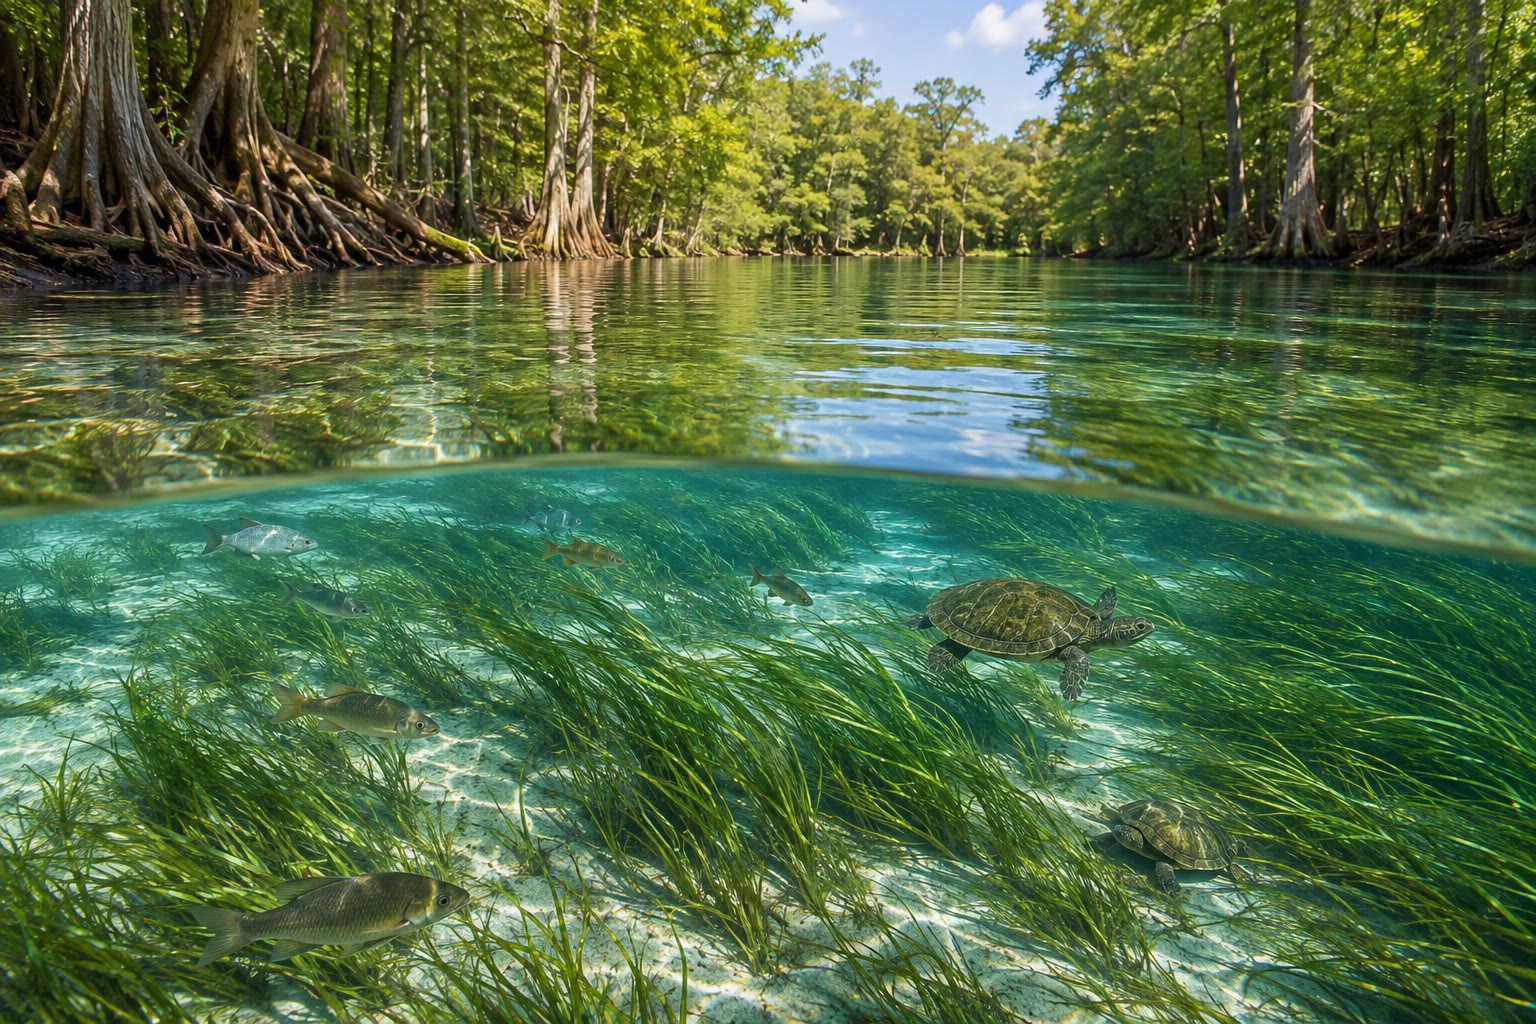
\includegraphics[width=0.6\linewidth]{images/book3/ai/b3-26-clear-spring.jpg}

{\small Sebuah mata air batu kapur: sebuah lapisan \omterm{def:b1:ecosystem-organization:trophic}{produsen} berupa
rumput belut dan alga dalam cahaya penuh, dan di atasnya \omterm{def:b1:ecosystem-organization:trophic}{konsumen} yang
untuknya anggaran energi ekologi yang pertama digambar.}
\end{omfigure}

\section{Alir energinya}

\begin{definition}[Produktivitas]\label{def:b1:ecosystem-organization:productivity}
\index{produktivitas primer}\index{produktivitas kasar}\index{produktivitas bersih}
Yang disebut \emph{produktivitas primer kasar} (GPP) sebuah \omterm{def:b1:ecosystem-organization:ecosystem}{ekosistem}
adalah laju \omterm{def:b1:ecosystem-organization:trophic}{produsennya} memancangkan energi lewat fotosintesis, tiap
satuan luas dan waktu (\unit{kJ.m^{-2}.yr^{-1}}, atau gram karbon atau
bahan kering); \emph{produktivitas primer bersih} (NPP) adalah apa
yang tersisa sesudah respirasi \omterm{def:b1:ecosystem-organization:trophic}{produsennya} sendiri --- bahan organik
yang benar-benar disediakan bagi bagian sistemnya yang lain.
\emph{Produktivitas sekunder} adalah laju \omterm{def:b1:ecosystem-organization:trophic}{konsumennya} membangun
biomassanya sendiri dari apa yang dimakannya. \emph{Biomassa} adalah
stok tegakannya, yaitu massa yang hadir pada sebuah saat;
produktivitasnya adalah sebuah alir, biomassanya sebuah simpanan, dan
nisbah keduanya adalah waktu pergantiannya.
\end{definition}

\begin{theorem}[Aturan sepuluh persen]\label{thm:b1:ecosystem-organization:lindeman}
\index{efisiensi trofik}
Dari energi yang memasuki satu \omterm{def:b1:ecosystem-organization:trophic}{aras trofik} sebagai makanan, hanya
sekitar sepersepuluh --- antara \qty{5}{} dan \qty{20}{\%} --- mencapai
aras berikutnya sebagai makanannya. Sisanya tidak dimakan, tidak
diasimilasi (pergi sebagai tinja), atau direspirasikan arasnya
sendiri. Karena itu energi yang tersedia turun sepuluh kali tiap
arasnya, yang menjadi sebab \omterm{def:b1:ecosystem-organization:foodweb}{rantai makanan} jarang melampaui empat atau
lima pautan, dan sebab biomassa dan jumlah pemangsa puncaknya kecil.
\end{theorem}
\begin{proof}[Bukti sebagian]
Energi yang diasimilasi sebuah aras adalah apa yang dimakannya
dikurangi apa yang dikeluarkannya; dari situ, respirasinya mengambil
apa yang dibelanjakan arasnya untuk hidup
(\cref{ch:b1:organism-environment}), dan hanya sisanya --- pertumbuhan
dan pembiakannya --- yang tersedia untuk dimakan. Tiap dari ketiga
fraksinya (dimakan, diasimilasi, diubah menjadi biomassa) jauh di
bawah satu: bagi seekor herbivora di sebuah padang rumput sekitar
\qty{20}{\%} pertumbuhan tumbuhannya dimakan, \qty{50}{\%} dari itu
diasimilasi, dan \qty{10}{\%} dari itu diubah menjadi daging, sehingga
memberi \qty{1}{\%}; bagi seekor karnivora, yang memakan dan
mengasimilasi lebih banyak mangsanya, sekitar \qty{10}{\%}. Aturannya
adalah sebuah keteraturan yang teramati, bukan sebuah hukum;
besarnya adalah apa yang diberikan pengukurannya.
\end{proof}
\begin{proof}[Bukti]
Lindeman (1942) mengukur, dalam sebuah danau kecil, energi yang
dipancangkan planktonnya dan energi yang dipegang serta
direspirasikan pada tiap aras di atasnya, lalu menemukan tiap arasnya
meneruskan sekitar sepersepuluh. Odum (1957) menggambar anggaran penuh
sebuah mata air Florida: dari \qty{1.7e6}{kcal} cahaya matahari tiap
meter persegi setahun, \omterm{def:b1:ecosystem-organization:trophic}{produsennya} memancangkan \num{20800} (kasar),
merespirasikan \num{12000} lalu meninggalkan \num{8800} bersih;
herbivoranya mengambil \num{3400} lalu meneruskan \num{380} kepada
karnivoranya; karnivoranya meneruskan \num{20} kepada karnivora
puncaknya. Dayagunanya adalah \qty{1.2}{\%}, \qty{16}{\%},
\qty{11}{\%} dan \qty{5}{\%} --- aturan sepuluh persennya dalam sebuah
faktor dua pada tiap langkahnya.
\end{proof}

\begin{omfigure}
\begin{tikzpicture}[font=\footnotesize, >=Stealth, line cap=round]
  % energy pyramid: widths proportional to log-ish scale of energy
  \fill[omExo!45] (-4.4,0) rectangle (4.4,0.9); \node at (0,0.45) {produsen: bersih \num{8800} kkal\,m$^{-2}$\,thn$^{-1}$ (kasar \num{20800})};
  \fill[omProp!45] (-2.9,1.1) rectangle (2.9,2.0); \node at (0,1.55) {herbivora: \num{3400} diambil, \num{1500} diasimilasi};
  \fill[omThm!45] (-1.5,2.2) rectangle (1.5,3.1); \node at (0,2.65) {karnivora: \num{380}};
  \fill[omDef!45] (-0.5,3.3) rectangle (0.5,4.2); \node[anchor=south] at (0,4.25) {karnivora puncak: \num{20}};
  \node[anchor=east, align=right] at (-4.6,0.45) {cahaya matahari:\\ \num{1700000}};
  \node[anchor=east, align=right, gray] at (-3.1,1.55) {\qty{16}{\%}};
  \node[anchor=east, align=right, gray] at (-1.7,2.65) {\qty{11}{\%}};
  \node[anchor=east, align=right, gray] at (-0.7,3.75) {\qty{5}{\%}};
  \draw[->, thick, gray] (4.6,0.45) -- (5.4,0.45) node[right, align=left] {respirasi dan\\ pengurai: panas};
  \draw[->, thick, gray] (3.1,1.55) -- (5.4,1.55); \draw[->, thick, gray] (1.7,2.65) -- (5.4,2.65); \draw[->, thick, gray] (0.7,3.75) -- (5.4,3.75);
\end{tikzpicture}

{\small Anggaran energi sebuah mata air (kilokalori tiap meter persegi
setahun). Tiap arasnya meneruskan sekitar sepersepuluh apa yang
diterimanya kepada yang berikutnya; sisanya pergi sebagai panas lewat
respirasi, sebagian besarnya lewat penguraiannya.}
\end{omfigure}

\begin{proposition}[Piramida]\label{prop:b1:ecosystem-organization:pyramids}
\index{piramida ekologi}
Menumpuk \omterm{def:b1:ecosystem-organization:trophic}{aras trofiknya} memberi sebuah \emph{piramida}. Sebuah
piramida \emph{energi} (alir tiap aras) selalu tegak: tiap arasnya
hanya dapat meneruskan lebih sedikit daripada yang diterimanya. Sebuah
piramida \emph{biomassa} (stok tegakan) biasanya tegak tetapi dapat
terbalik: di laut lepas fitoplanktonnya, yang dimakan secepat ia
tumbuh, berbobot lebih ringan pada tiap saat daripada zooplankton yang
hidup darinya, sebab ia berganti dalam beberapa hari sedangkan
hewannya bertahan berbulan-bulan. Sebuah piramida \emph{cacah} dapat
berbentuk apa saja: satu pohon ek memberi makan ribuan ulat. Energilah
ukuran yang jujur.
\end{proposition}

\begin{method}[Menyusun sebuah anggaran energi]\label{met:b1:ecosystem-organization:budget}
\begin{enumerate}
  \item Ukurlah GPP: lewat pertukaran gasnya (oksigen yang dilepaskan
        atau $\mathrm{CO_2}$ yang diserap sebuah petak atau sebuah
        botol dalam terang dan gelap: terang dikurangi gelap memberi
        yang kasar, terang saja memberi yang bersih), atau lewat
        panennya (biomassa yang diperoleh tiap tahun ditambah apa yang
        dimakan dan digugurkan).
  \item Ukurlah, bagi tiap aras \omterm{def:b1:ecosystem-organization:trophic}{konsumennya}, asupannya (apa yang
        dimakannya), asimilasinya (asupan dikurangi tinja),
        respirasinya (pemakaian oksigennya) dan produksinya
        (pertumbuhan ditambah anaknya $=$ asimilasi dikurangi
        respirasi).
  \item \omterm{thm:b1:ecosystem-organization:lindeman}{Efisiensi trofik} antararas $=$ produksi aras atasnya $/$
        produksi aras bawahnya. Periksalah bahwa respirasi ditambah
        produksi ditambah penguraian tiap arasnya berjumlah sama dengan
        asimilasinya.
  \item Ubahlah menjadi satuan bersama (\unit{kJ}, atau gram karbon
        pada sekitar \qty{40}{kJ/g}) lalu gambarlah piramidanya; jumlah
        seluruh respirasinya seharusnya mendekati GPP-nya sepanjang
        setahun dalam sebuah \omterm{def:b1:ecosystem-organization:ecosystem}{ekosistem} yang mantap.
\end{enumerate}
\end{method}

\begin{example}[Mengapa puncaknya tipis]\label{ex:b1:ecosystem-organization:top}
Sekilometer persegi sabana membuat sekitar \qty{5000}{t} rumput
setahun; pemakan rumputnya mengubahnya menjadi \qty{50}{t} antelop dan
kerbau; singanya menjadi \qty{2}{t} singa --- satu atau dua ekor. Untuk
memberi makan seekor harimau, sebuah hutan harus cukup besar sehingga
sepersepuluh dari sepersepuluh dari sepersepuluh cahaya mataharinya
menjadi seekor rusa utuh tiap pekan: seratus kilometer persegi tiap
harimau, yang menjadi sebab karnivora besar itu jarang, menjelajah
jauh, lalu lenyap lebih dahulu ketika \omterm{def:b1:ecosystem-organization:niche}{habitatnya} mengecil.
\end{example}

\begin{proposition}[Produktivitas biomanya]\label{prop:b1:ecosystem-organization:biomes}
\index{bioma}
\omterm{def:b1:ecosystem-organization:productivity}{Produktivitas primer} bersih tiap satuan luas ditetapkan cahaya, suhu,
air dan haranya: hutan hujan tropis \qtyrange{2000}{3500}{} g bahan
kering tiap meter persegi setahun; hutan sedang dan lahan budi daya
\qtyrange{600}{1500}{}; padang rumput \qtyrange{200}{1500}{}; tundra
dan gurun di bawah \qty{200}{}; laut terbuka sekitar \qty{125}{}
(cahayanya berlimpah, haranya langka), pantai penaikan air dan terumbu
\qtyrange{500}{2500}{}. Samudranya, dua pertiga planetnya, menyumbang
sekitar separuh produksi globalnya; hutannya, sepersepuluh daratannya,
menyumbang sepertiga produksi daratannya. Tempat air dan haranya
berlimpah, produktivitasnya mengikuti cahaya dan hangatnya; tempat
keduanya tidak, ia mengikuti keduanya.
\end{proposition}

\begin{omfigure}
\begin{tikzpicture}
\begin{axis}[
  xbar, bar width=8pt,
  width=0.84\linewidth, height=6.6cm,
  axis x line=bottom, axis y line=left,
  xmin=0, xmax=2600, xlabel={produktivitas primer bersih (\unit{g.m^{-2}.yr^{-1}}, bahan kering)},
  xlabel style={font=\small, at={(axis description cs:0.5,-0.12)}, anchor=north},
  symbolic y coords={gurun, laut terbuka, tundra, padang rumput sedang, lahan budi daya, hutan sedang, muara dan terumbu, hutan hujan tropis},
  ytick=data, tick label style={font=\small},
  enlarge y limits=0.08, xtick={0,500,1000,1500,2000,2500},
  nodes near coords, nodes near coords style={font=\scriptsize, anchor=west},
]
\addplot[fill=omExo!45, draw=omExo] coordinates {(90,gurun) (125,laut terbuka) (140,tundra) (600,padang rumput sedang) (650,lahan budi daya) (1200,hutan sedang) (1800,muara dan terumbu) (2200,hutan hujan tropis)};
\end{axis}
\end{tikzpicture}

{\small \omterm{def:b1:ecosystem-organization:productivity}{Produktivitas primer} bersih purata bioma utamanya. Sebuah
jangkau dua puluh kali lipat, yang ditetapkan air, hangat, cahaya dan
haranya.}
\end{omfigure}

\begin{omfigure}
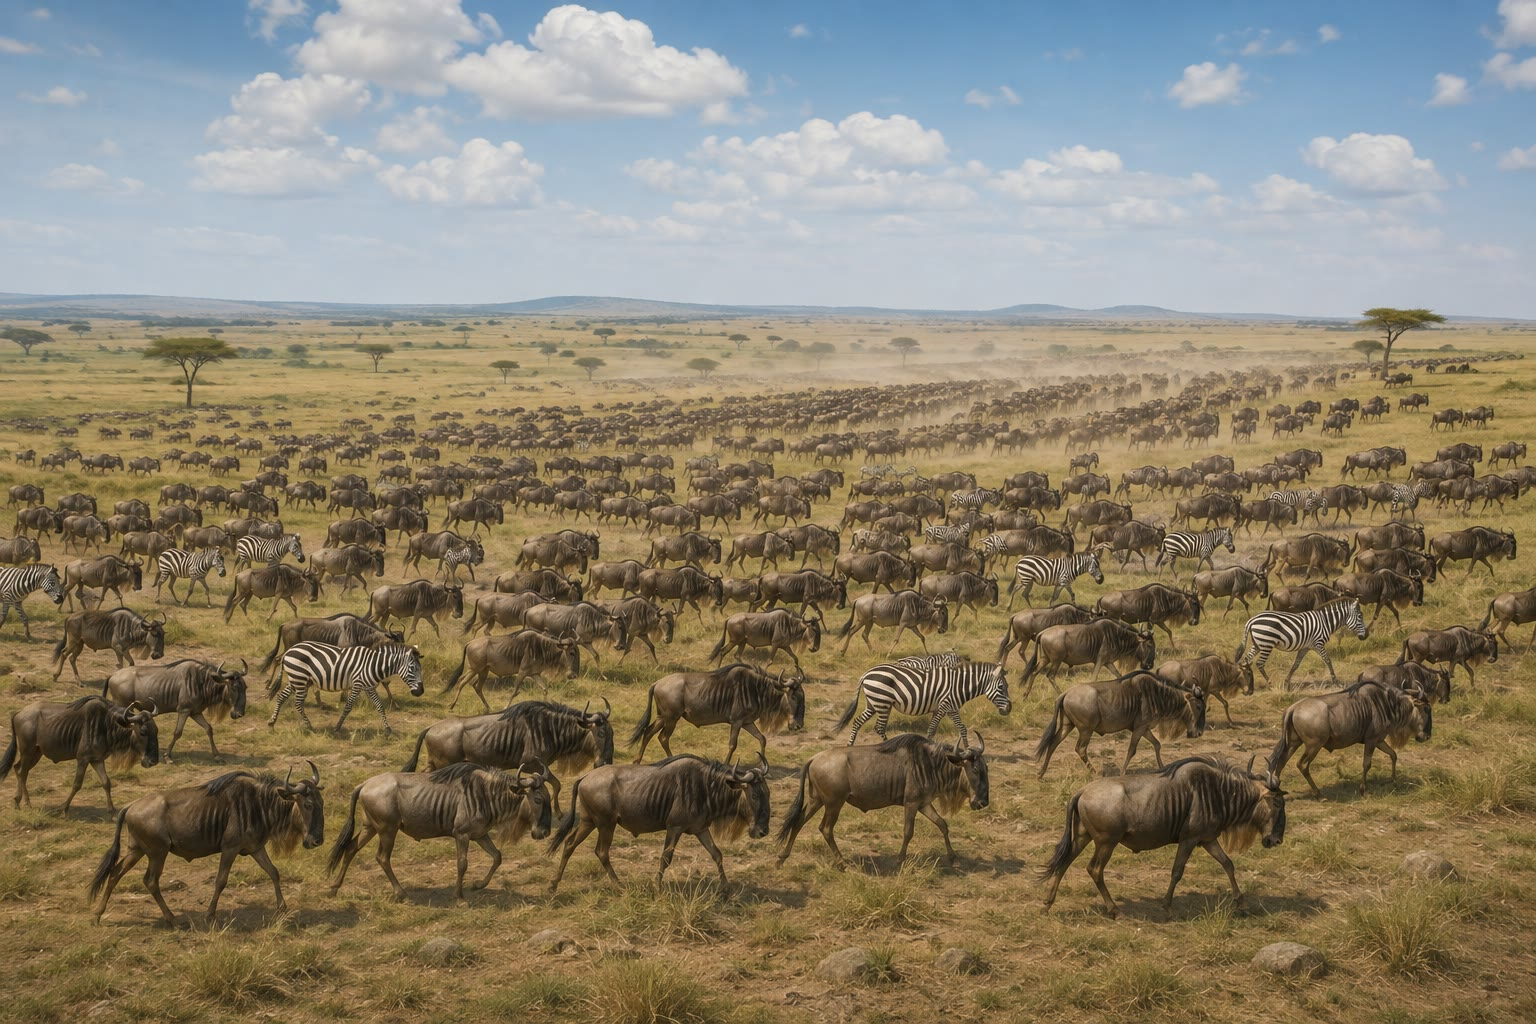
\includegraphics[width=0.6\linewidth]{images/book3/ai/b3-26-wildebeest-migration.jpg}

{\small Pemakan rumput di sebuah sabana: sebuah aras \omterm{def:b1:ecosystem-organization:trophic}{konsumen} primer
berisi sejuta hewan, yang mengikuti hujan yang menetapkan
produktivitas rumputnya, lalu membawa sepersepuluh energinya kepada
pemangsa di belakangnya.}
\end{omfigure}

\section{Menghitung keanekaragaman}

\begin{definition}[Kekayaan spesies, indeks keanekaragaman]\label{def:b1:ecosystem-organization:diversity}
\index{kekayaan spesies}\index{indeks Shannon}
Yang disebut \emph{kekayaan spesies} $S$ sebuah \omterm{def:b1:ecosystem-organization:ecosystem}{komunitas} adalah cacah
spesies di dalamnya. Kekayaannya saja mengabaikan kelimpahannya:
sebuah hutan dengan seratus pohon ek dan satu dari tiap sembilan pohon
lain kurang beranekaragam daripada sebuah hutan dengan sepuluh dari
tiap jenisnya. Yang disebut \emph{indeks Shannon}
\[
H = -\sum_{i=1}^{S} p_i \ln p_i ,
\]
dengan $p_i$ adalah fraksi individu yang tergolong spesies $i$, naik
bersama kekayaan maupun \emph{kemerataan}nya; ia bernilai $\ln S$
ketika seluruh spesiesnya sama melimpah dan mendekati nol ketika satu
mendominasi. \emph{Kemerataan}nya adalah $H/\ln S$. Keanekaragamannya
umumnya naik dari kutub ke tropisnya, bersama luasnya, bersama waktu
sejak gangguan terakhirnya, dan bersama produktivitas tapaknya sampai
sebuah titik.
\end{definition}

\begin{method}[Mencuplik sebuah komunitas]\label{met:b1:ecosystem-organization:sampling}
\begin{enumerate}
  \item Cupliklah dengan sebuah cara yang sesuai bagi \omterm{def:b1:organism-environment:organism}{organismenya}
        (kuadrat, jaring, perangkap, transek) lalu catatlah cacah
        individu tiap spesiesnya.
  \item Gambarkan cacah spesies yang ditemukan terhadap cacah
        cuplikannya (atau individunya): kurvanya naik curam, lalu
        mendatar; tempat ia mendatar, kekayaannya nyaris lengkap.
        Bandingkan \omterm{def:b1:ecosystem-organization:ecosystem}{komunitasnya} hanya pada upaya cuplikan yang setara.
  \item Hitunglah $H$ dan kemerataannya; bandingkan dengan gambar
        peringkat--kelimpahannya (spesies diperingkat menurut
        kelimpahannya, pada sebuah skala logaritmik), yang
        kemiringannya memperlihatkan dominasinya.
  \item Tafsirkan: kemerataan yang rendah menunjuk pada sebuah spesies
        yang mendominasi atau sebuah cekaman; turunnya $H$ sepanjang
        waktu menunjuk pada sebuah perubahan dalam \omterm{def:b1:ecosystem-organization:ecosystem}{biotopnya}.
\end{enumerate}
\end{method}

\begin{example}[Dua hutan]\label{ex:b1:ecosystem-organization:twowoods}
Hutan A: 100 pohon ek dan satu dari tiap sembilan pohon lain; $H = -(0.917\ln
0.917 + 9\times 0.0092\ln 0.0092) = 0.08 + 0.39 = 0.47$, kemerataannya
$0.47/2.30 = 0.20$. Hutan B: sepuluh dari tiap sepuluh spesies yang sama; $H =
\ln 10 = 2.30$, kemerataannya 1. Kekayaan yang sama, lima kali keanekaragamannya.
\end{example}

\section{Latihan}

\begin{exercise}[$\star$]\label{exo:b1:ecosystem-organization:1}
Definisikan \omterm{def:b1:ecosystem-organization:ecosystem}{ekosistem}, \omterm{def:b1:ecosystem-organization:ecosystem}{komunitas} dan \omterm{def:b1:ecosystem-organization:ecosystem}{biotop}, dengan contoh sebuah kolam.
\end{exercise}

\begin{exercise}[$\star$]\label{exo:b1:ecosystem-organization:2}
Bedakan \omterm{def:b1:ecosystem-organization:niche}{habitat} dari \omterm{def:b1:ecosystem-organization:niche}{relung}, dan \omterm{def:b1:ecosystem-organization:niche}{relung} dasar dari \omterm{def:b1:ecosystem-organization:niche}{relung} nyata.
\end{exercise}

\begin{exercise}[$\star$]\label{exo:b1:ecosystem-organization:3}
Dari piramida energi mata airnya, hitunglah dayaguna dari cahaya
matahari ke produksi kasarnya, dan fraksi produksi bersihnya yang
diambil herbivoranya.
\end{exercise}

\begin{exercise}[$\star$]\label{exo:b1:ecosystem-organization:4}
Sebutkan keempat kelompok trofiknya lalu katakan yang mana yang
menutup daur materinya.
\end{exercise}

\begin{exercise}[$\star\star$]\label{exo:b1:ecosystem-organization:5}
NPP sebuah padang rumput adalah \qty{800}{g.m^{-2}.yr^{-1}}
(\qty{17}{kJ/g}). Kelinci memakan \qty{15}{\%}-nya, mengasimilasi
\qty{50}{\%} apa yang dimakannya, lalu mengubah \qty{5}{\%} apa yang
diasimilasinya menjadi kelinci. Hitunglah produksi kelincinya tiap
hektar dan \omterm{thm:b1:ecosystem-organization:lindeman}{efisiensi trofik} dari NPP ke kelincinya.
\end{exercise}

\begin{exercise}[$\star\star$]\label{exo:b1:ecosystem-organization:6}
Jelaskan mengapa sebuah piramida biomassa dapat terbalik di lautnya
tetapi sebuah piramida energi tak pernah demikian.
\end{exercise}

\begin{exercise}[$\star\star$]\label{exo:b1:ecosystem-organization:7}
Hitunglah \omterm{def:b1:ecosystem-organization:diversity}{indeks Shannon} dan kemerataan bagi sebuah cuplikan berisi 50
A, 30 B, 15 C dan 5 D. Bandingkan dengan empat spesies pada 25
masing-masing.
\end{exercise}

\begin{exercise}[$\star\star$]\label{exo:b1:ecosystem-organization:8}
Dalam sebuah percobaan botol terang dan gelap, oksigen dalam botol
terangnya naik \qty{3}{mg/L} dalam sehari dan dalam botol gelapnya
turun \qty{1}{mg/L}. Hitunglah \omterm{def:b1:ecosystem-organization:productivity}{produktivitas kasar} dan bersih airnya
dalam miligram oksigen tiap liter tiap hari, dan dalam gram karbon
(\qty{1}{g} $\mathrm{O_2}$ $\approx$ \qty{0.375}{g} C).
\end{exercise}

\begin{exercise}[$\star\star$]\label{exo:b1:ecosystem-organization:9}
Mengapa tak ada \omterm{def:b1:ecosystem-organization:foodweb}{rantai makanan} sepuluh pautan, dan mengapa pulau dan
gurun memiliki rantai yang lebih pendek daripada hutan?
\end{exercise}

\begin{exercise}[$\star\star\star$]\label{exo:b1:ecosystem-organization:10}
Seorang manusia dapat memakan biji-bijiannya langsung atau
memberikannya kepada sapinya. Dengan \omterm{thm:b1:ecosystem-organization:lindeman}{efisiensi trofik} \qty{10}{\%} bagi
sapinya, hitunglah lahan yang dibutuhkan untuk memberi makan satu orang
dengan daging sapi lawan dengan biji-bijian bila ladangnya
menghasilkan \qty{6}{t} biji-bijian tiap hektar dan seseorang
memerlukan \qty{1}{t} setahun. Apa yang dikatakan hal ini tentang \omterm{def:b1:ecosystem-organization:trophic}{aras
trofik} manusia dan \omterm{thm:b1:populations:logistic}{daya dukung} planetnya?
\end{exercise}

\begin{exercise}[$\star\star\star$]\label{exo:b1:ecosystem-organization:11}
Laut terbuka memiliki NPP yang rendah tiap meter persegi tetapi
separuh produksi dunianya. Damaikanlah keduanya, lalu jelaskan mengapa
perikanan lautnya memusat pada beberapa persen luasnya.
\end{exercise}

\begin{exercise}[$\star\star\star$]\label{exo:b1:ecosystem-organization:12}
``Sebuah \omterm{def:b1:ecosystem-organization:ecosystem}{ekosistem} adalah sebuah mesin untuk mengubah cahaya matahari
menjadi panas, dengan kehidupan sebagai hasil sampingannya.'' Bahaslah
dalam satu paragraf: alir energi lawan daur materi, apa yang dilakukan
penguraiannya, dan apa yang ditinggalkan kalimat itu.
\end{exercise}

\section{Soal: Anggaran Sebuah Mata Air}

\begin{problem}[{Soal akhir pekan --- mata air Odum yang disusun aras
demi aras: cahaya matahari ke rumputnya, rumput ke siputnya, siput ke
ikannya, ikan ke bangaunya, dengan respirasi dan penguraiannya,
berakhir pada efisiensi trofik pada tiap arasnya}]
\label{pb:b1:ecosystem-organization:1}
Sebuah mata air menerima \qty{1.7e6}{kcal} cahaya matahari tiap meter
persegi setahun. \omterm{def:b1:ecosystem-organization:trophic}{Produsennya} memancangkan \qty{20800}{kcal} (kasar)
lalu merespirasikan \qty{12000}{}. Herbivoranya memakan
\qty{3400}{kcal} bahan tumbuhan, yang \qty{1500}{} di antaranya
diasimilasinya, \qty{1100}{} direspirasikannya, dan sisanya diubahnya
menjadi pertumbuhan dan anaknya. Karnivoranya memakan \qty{380}{kcal},
merespirasikan \qty{300}{} lalu menghasilkan sisanya; karnivora
puncaknya memakan \qty{20}{kcal}, merespirasikan \qty{14}{} lalu
menghasilkan \qty{6}{}. Segala yang tidak dimakan atau direspirasikan
pergi ke penguraiannya, yang merespirasikannya. Ambillah
\qty{1}{kcal} $= \qty{4.18}{kJ}$ dan \qty{10}{kcal} tiap gram biomassa
kering.

\medskip
\noindent\textbf{Bagian I --- \omterm{def:b1:ecosystem-organization:trophic}{Produsennya}.}
\begin{enumerate}
  \item Hitunglah \omterm{def:b1:ecosystem-organization:productivity}{produktivitas primer} bersihnya.
  \item Hitunglah dayaguna fotosintesisnya: produksi kasar dibagi
        cahaya mataharinya. Bandingkanlah dengan \qty{34}{\%} pada
        \cref{ch:b1:photosynthesis} lalu sebutkan tiga kehilangan yang
        memisahkan keduanya.
  \item Berapa fraksi produksi kasarnya yang direspirasikan
        \omterm{def:b1:ecosystem-organization:trophic}{produsennya}?
  \item Berapa banyak produksi bersihnya yang dimakan herbivoranya, dan
        berapa banyak yang langsung pergi ke penguraiannya?
  \item Nyatakan NPP-nya dalam gram bahan kering tiap meter persegi
        setahun lalu tempatkanlah mata airnya di antara bioma dalam bab
        ini.
  \item Berapa banyak cahaya mataharinya, tiap meter persegi dan
        setahun, yang meninggalkan mata airnya sebagai panas tanpa
        pernah melewati sebuah \omterm{def:b1:organism-environment:organism}{organisme} hidup?
\end{enumerate}

\medskip
\noindent\textbf{Bagian II --- \omterm{def:b1:ecosystem-organization:trophic}{Konsumennya}.}
\begin{enumerate}[resume]
  \item Hitunglah produksi herbivoranya dan dayaguna asimilasinya
        (yang diasimilasi dibagi yang dimakan).
  \item Hitunglah dayaguna produksi herbivoranya (produksi dibagi yang
        diasimilasi).
  \item Hitunglah \omterm{thm:b1:ecosystem-organization:lindeman}{efisiensi trofik} dari \omterm{def:b1:ecosystem-organization:trophic}{produsen} ke herbivoranya:
        produksi herbivoranya dibagi produksi primer bersihnya.
  \item Hitunglah produksi karnivoranya dan \omterm{thm:b1:ecosystem-organization:lindeman}{efisiensi trofik} dari
        herbivora ke karnivoranya.
  \item Hitunglah \omterm{thm:b1:ecosystem-organization:lindeman}{efisiensi trofik} dari karnivora ke karnivora
        puncaknya.
  \item Berapa banyak energi tiap meter persegi setahun yang mencapai
        \omterm{def:b1:body-plans-tissues:tissue}{jaringan} karnivora puncaknya sendiri? Berapa fraksi cahaya
        mataharinya itu?
  \item Mengapa dayaguna asimilasinya naik dari herbivora ke
        karnivoranya?
\end{enumerate}

\medskip
\noindent\textbf{Bagian III --- Penguraiannya dan neracanya.}
\begin{enumerate}[resume]
  \item Sebutkan tiap alir ke penguraiannya (produksi bersih yang tak
        dimakan, tinja herbivoranya dan produksi herbivora yang tak
        dimakan, dan seterusnya) lalu jumlahkanlah.
  \item Hitunglah respirasi total \omterm{def:b1:ecosystem-organization:ecosystem}{ekosistemnya}: \omterm{def:b1:ecosystem-organization:trophic}{produsen}, herbivora,
        karnivora, karnivora puncak dan penguraiannya.
  \item Bandingkanlah dengan produksi kasarnya. Apa arti perbandingannya
        bagi biomassa mata airnya sepanjang setahun?
  \item Berapa fraksi produksi kasarnya yang direspirasikan
        penguraiannya?
  \item Gambarlah piramida energinya dengan produksi keempat arasnya
        lalu berilah label dayagunanya.
\end{enumerate}

\medskip
\noindent\textbf{Bagian IV --- Simpanan, pergantian dan perubahan.}
Biomassa tegakannya adalah \qty{800}{g/m^2} \omterm{def:b1:ecosystem-organization:trophic}{produsen}, \qty{40}{g/m^2}
herbivora, \qty{10}{g/m^2} karnivora dan \qty{1.5}{g/m^2} karnivora
puncak.
\begin{enumerate}[resume]
  \item Ubahlah tiap biomassanya menjadi kilokalori lalu gambarlah
        piramida biomassanya. Adakah ia tegak?
  \item Hitunglah waktu pergantian (biomassa dibagi produksi) tiap
        arasnya. Yang mana yang berganti paling cepat, dan mengapa?
  \item Seekor bangau seberat \qty{2}{kg} hidup dari produksi karnivora
        puncak mata airnya. Berapa meter persegi yang diperlukannya?
  \item Mata airnya diperkaya pupuk dan produksi kasarnya berlipat dua,
        tetapi herbivoranya tak sanggup makan lebih cepat. Apa yang
        terjadi pada produksi tambahannya, pada respirasi
        penguraiannya, dan pada oksigen airnya pada malam hari?
  \item Sebuah ikan baru dimasukkan yang memakan telur herbivoranya
        lalu memaruhkan produksinya. Ramalkan produksi karnivoranya dan
        jumlah bangaunya, serta nasib rumput belutnya.
  \item Jelaskan mengapa menyingkirkan karnivora puncaknya akan
        mengubah rumput belutnya jauh lebih banyak daripada
        menyingkirkan herbivora yang senilai energi yang sama.
  \item Nyatakan hasilnya: \omterm{thm:b1:ecosystem-organization:lindeman}{efisiensi trofik} pada tiap dari ketiga
        pemindahannya, dayaguna dari cahaya matahari ke produksi
        kasarnya, dan fraksi energi mataharinya yang mencapai karnivora
        puncaknya.
\end{enumerate}
\end{problem}
